
\documentclass[11pt]{article}

\usepackage[bottom]{footmisc}
\usepackage{courier}
\usepackage{graphicx}
\usepackage[hidelinks]{hyperref}
\usepackage{amsmath,amsfonts,amssymb,geometry,bm}
\geometry{top=2cm}
\usepackage{enumerate}

% -------- Title Info
\title{CS201 Markov Project Analysis}
\author{Keping Wang (netid: kw238)}


% -------- The Document
\begin{document}
\maketitle

\section{How I did the benchmark}
It is hard to write an accurate benchmark on the JVM because JVM is an adaptive virtual machine which automatically does optimizations for the source code.\footnote{\url{http://www.oracle.com/technetwork/articles/java/architect-benchmarking-2266277.html}}

The \texttt{BenchMark.java} file provided by the instructor doesn't avoid containing flaws in benchmarking, for example:
\begin{enumerate}
\item It lacks warm up rounds. I do not fully understand how JVM and CPU work, but the running time of a piece of good does show great volatility in the first several iterations.
\item It uses unnecessary multithreading. If I want an accurate benchmark for a piece of code, I would really be willing to sacrifice some of my time waiting in front of the computer in exchange for a guaranteed accurate measurement. Multithreading just affects the running time measurement too much. When the number of threads exceeds the number of CPU cores, the threads are slowed down a lot. And when some threads are finished first, the remaining threads will be allocated with more computing power. A fixed thread pool is perhaps better, but still not something that I would use.
\item The running time of \texttt{.setTraining()} and \texttt{.getRandomText} are measured together (with the confusion of threads), but they could be measured separately.
\item The JVM might have done some optimizations which haven't been taken into account by \texttt{BenchMark.java}. But I'm not sure about this.
\end{enumerate}

So the recommended way to write benchmarks for a person without comprehensive knowledge of the JVM is to use a well written framework. Here I chose JMH (Java Microbenchmark Harness)\footnote{\url{http://openjdk.java.net/projects/code-tools/jmh/}}, which basically works by generating synthetic benchmark code by reading annotations in the source code.

To use JMH, I had to create a separate Maven project for benchmarking. I wrote \texttt{MarkovBench.java} and \texttt{MapBench.java} respectively to benchmark the time of the Markov model and map insertion. Besides, I made the original \texttt{markov-start-fall16} a Maven project so that I could easily add it as a dependency in my benchmarking Maven project.

One thing to note about measuring \texttt{.getRandomText(int T)} is that this method is not always generating a text of size T. To test the running time of generating T characters, if the call stops before generating the required length, I iteratively call $\texttt{.getRandomText()}$ until all T length is generated.

JMH automatically generated benchmark output. I directed the output into CSV files and then visualized the results using Python \texttt{pandas} and \texttt{matplotlib}. The Python code is in \texttt{analysis/BenchAnalysis.ipynb}.

What follows is the running time analysis of the Markov model in section 2 and map insertion in section 3. A preview of the conclusion: all the hypotheses made in the google doc are true.

\section{Markov Time Analysis}

All the running time is illusated with graphs. For all the following graphs, the y axis is the running time in milliseconds ($10^{-3}$s), and the blue shades in all the following graphs are $99.9\%$ confidence intervals. The benchmarks with respect to $N$ and $T$ use 6-grams $k=6$. The source training text is \texttt{hawthorne.txt}.

The \texttt{\bf .setTraining()} method in \texttt{\bf BruteMarkov} is $O(1)$ since it does nothing other than passing a reference.

\centerline{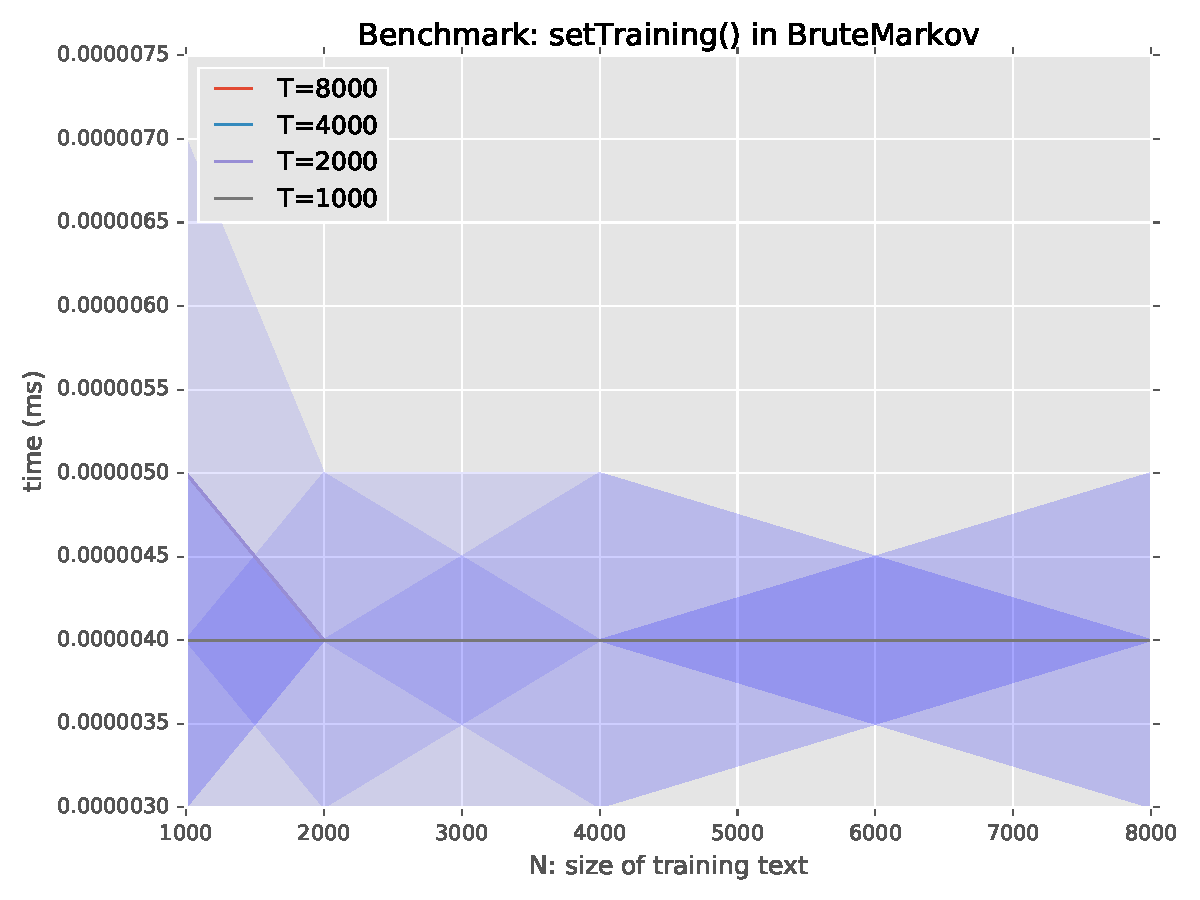
\includegraphics[width=0.6\linewidth]{setTraining_BruteMarkov_N.pdf}}

The \texttt{\bf .getRandomText()} method in \texttt{\bf BruteMarkov} is $O(NT)$, which means the running time is proportional to $N$ and proportional to $T$.

\centerline{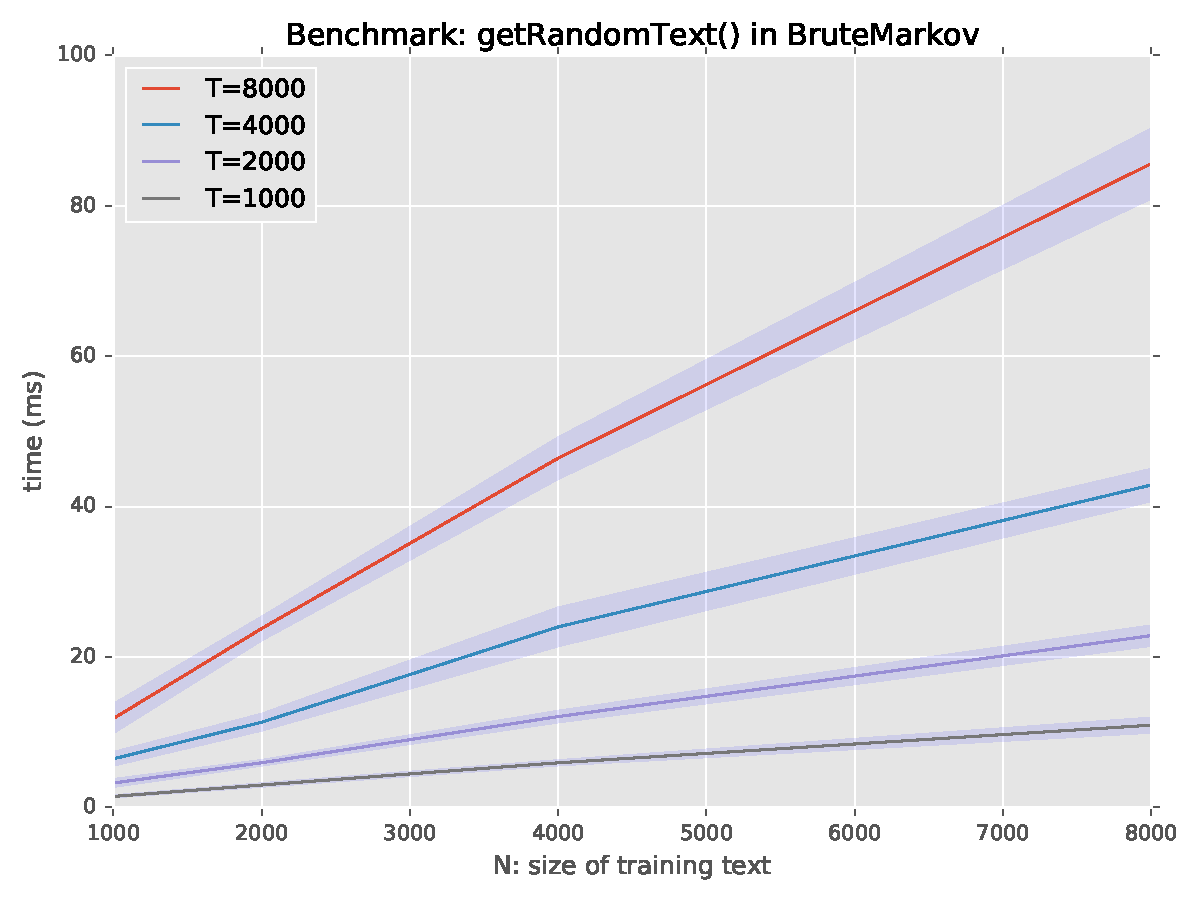
\includegraphics[width=0.6\linewidth]{getRandomText_BruteMarkov_N.pdf}}

\centerline{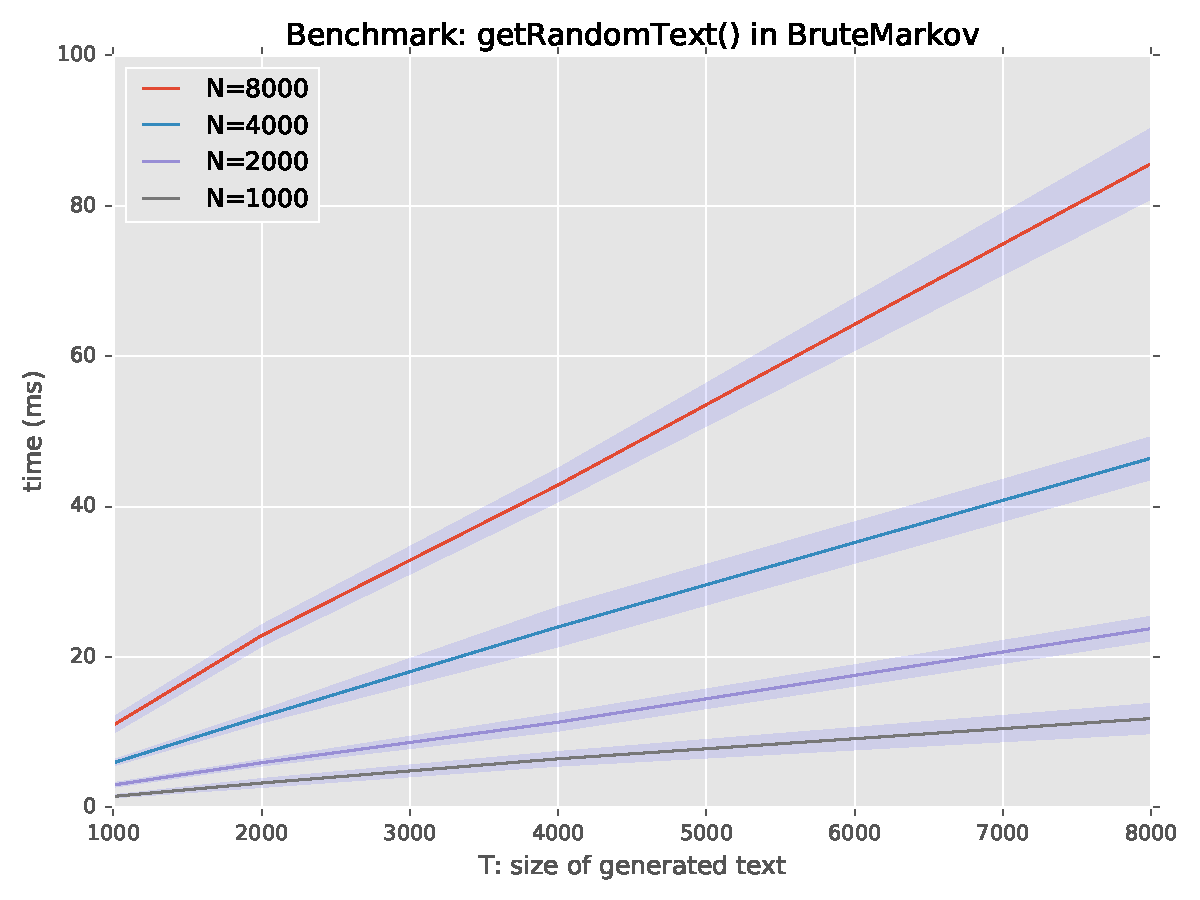
\includegraphics[width=0.6\linewidth]{getRandomText_BruteMarkov_T.pdf}}

The \texttt{\bf .setTraining()} method in \texttt{\bf EfficientMarkov} is $O(N)$.

\centerline{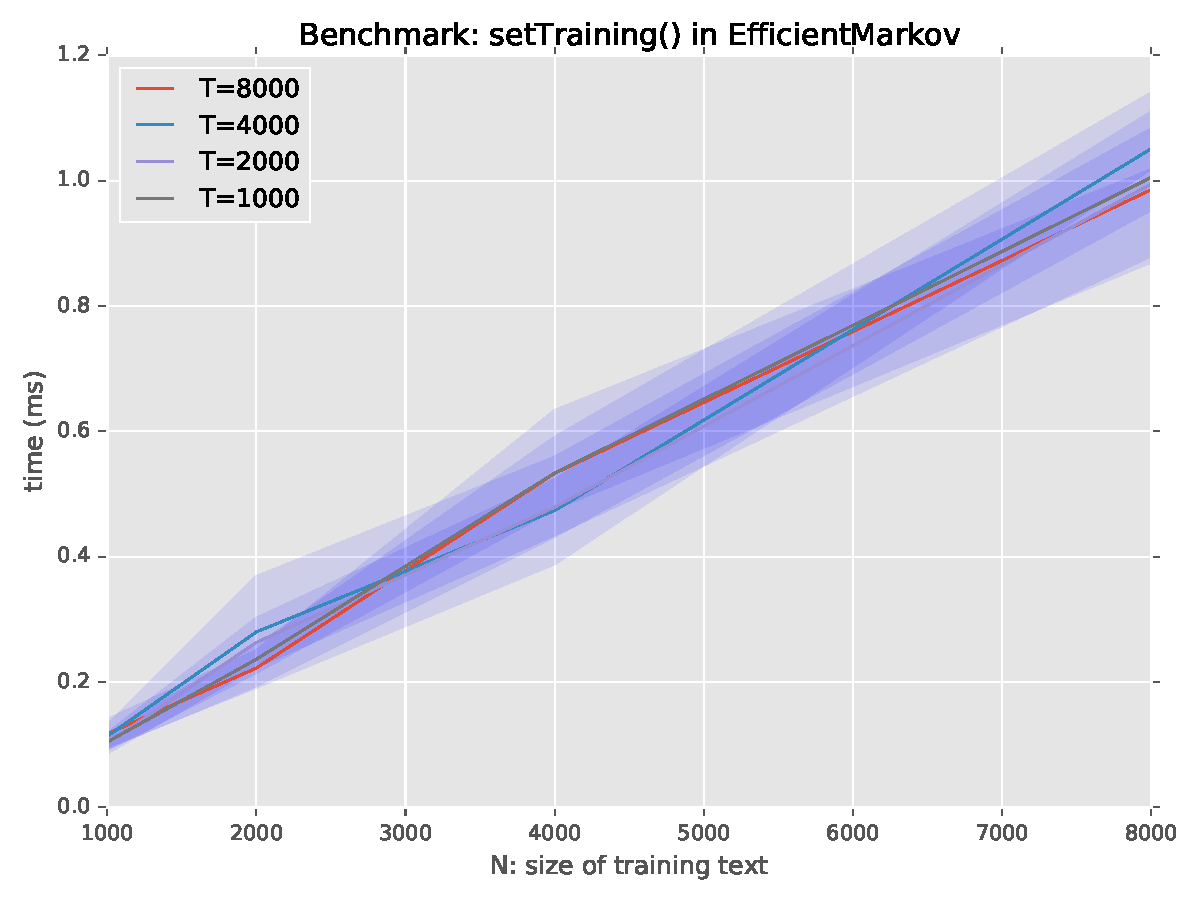
\includegraphics[width=0.6\linewidth]{setTraining_EfficientMarkov_N.pdf}}

\centerline{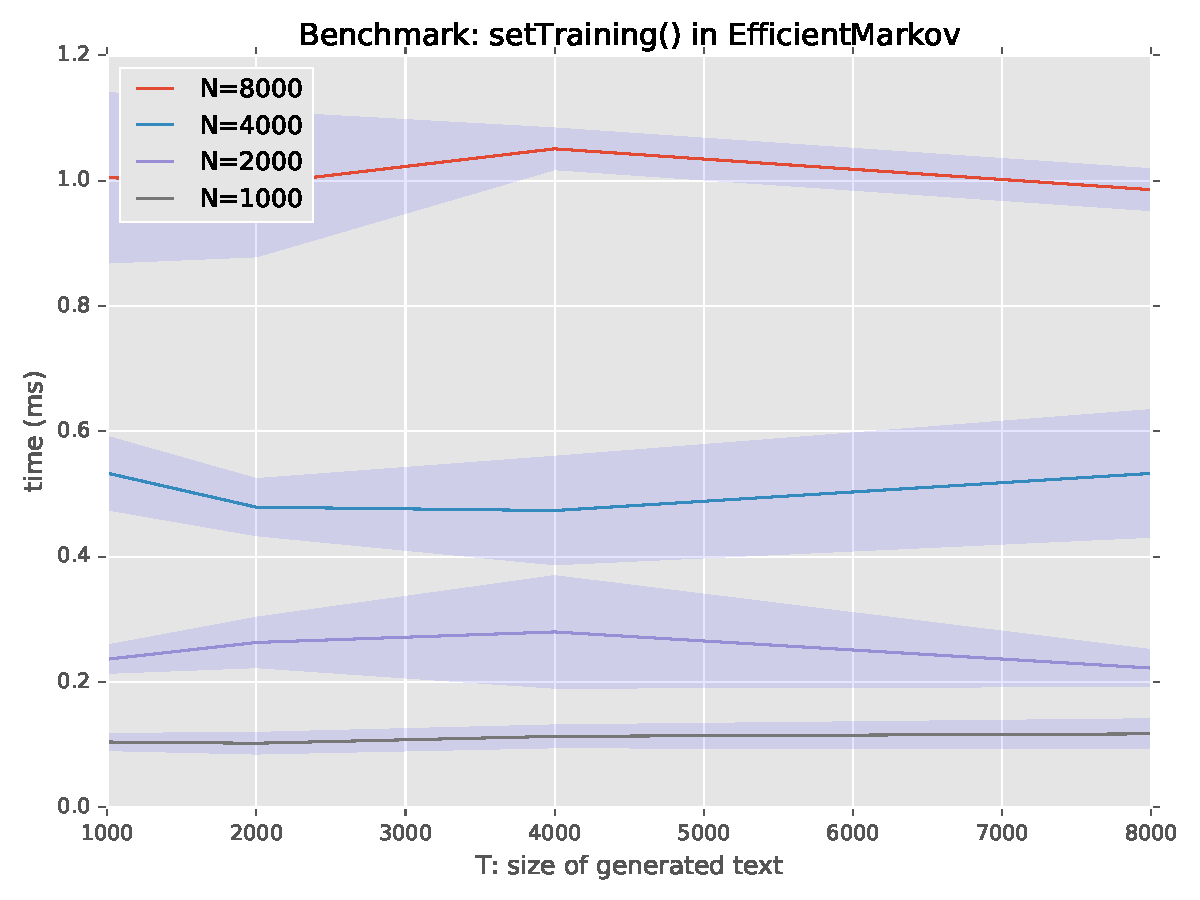
\includegraphics[width=0.6\linewidth]{setTraining_EfficientMarkov_T.pdf}}

The \texttt{\bf .getRandomText()} method in \texttt{\bf EfficientMarkov} is $O(T)$.

\centerline{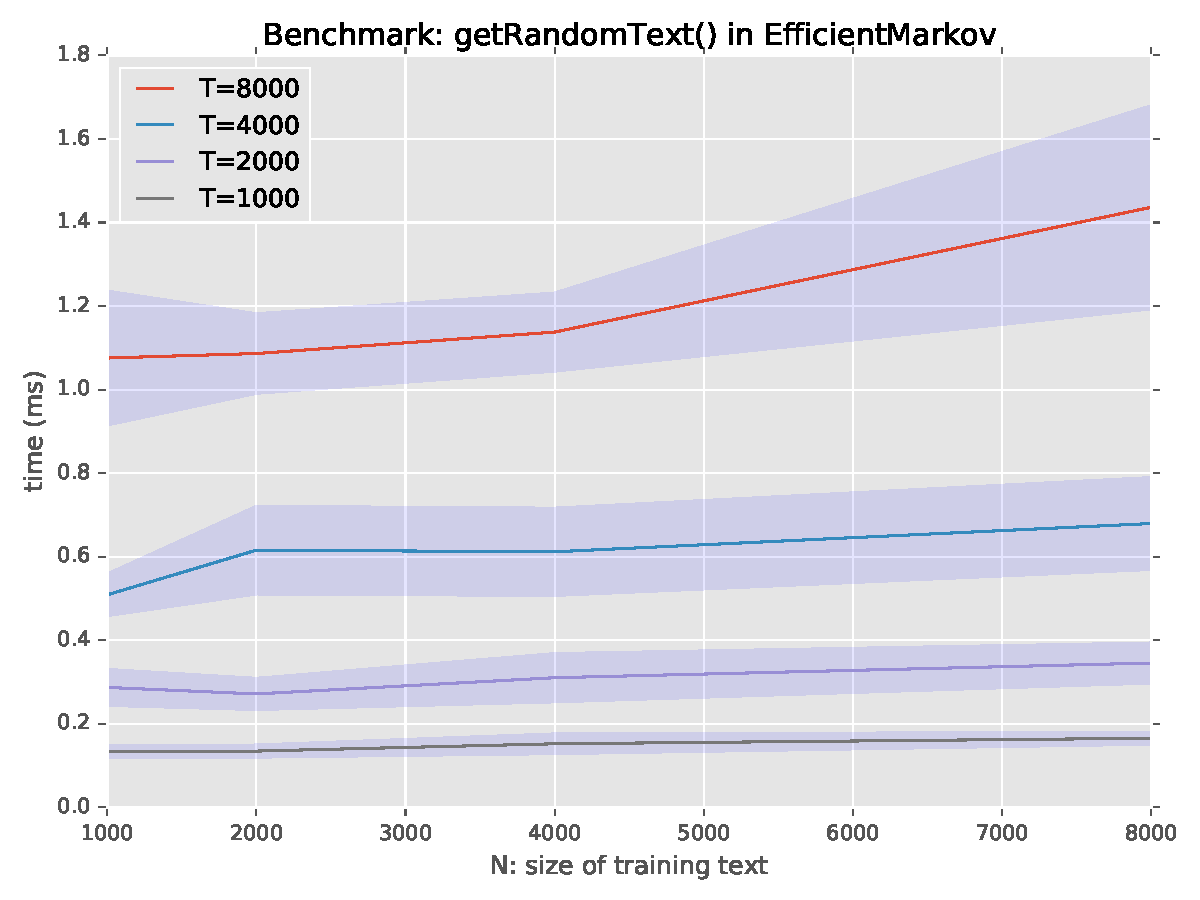
\includegraphics[width=0.6\linewidth]{getRandomText_EfficientMarkov_N.pdf}}

\centerline{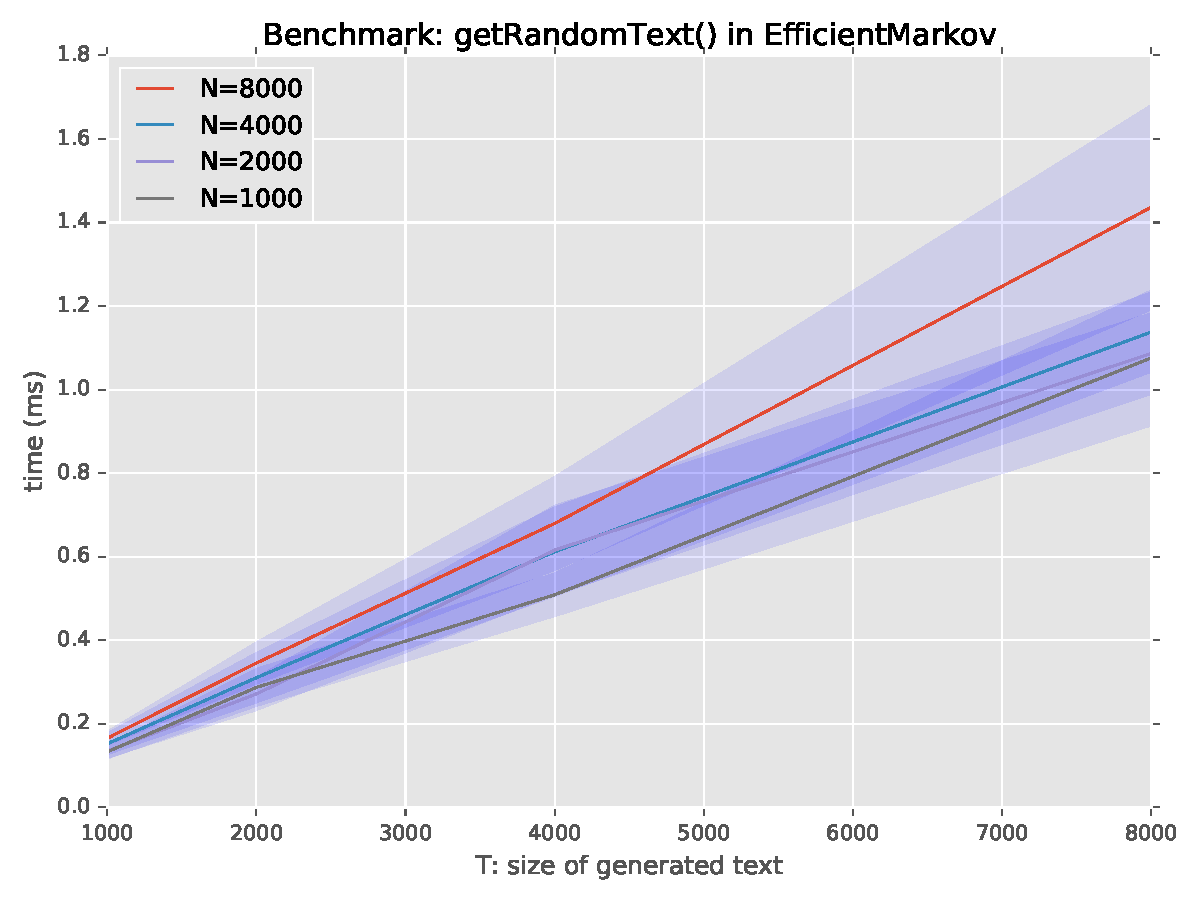
\includegraphics[width=0.6\linewidth]{getRandomText_EfficientMarkov_T.pdf}}

As for $k$, the running time of some methods are related to $k$, and the specific relationship depends on the source text used for training. However, all the methods have running time independent of $k$ asymptotically. These graphs has $N=4000$ and $T=4000$. (The running time of \texttt{.setTraining()} in \texttt{BruteMarkov} is so close to $0$ that we cannot see the line when it is ploted in the same graph as \texttt{.setTrainig()} in \texttt{EfficientMarkov})

\centerline{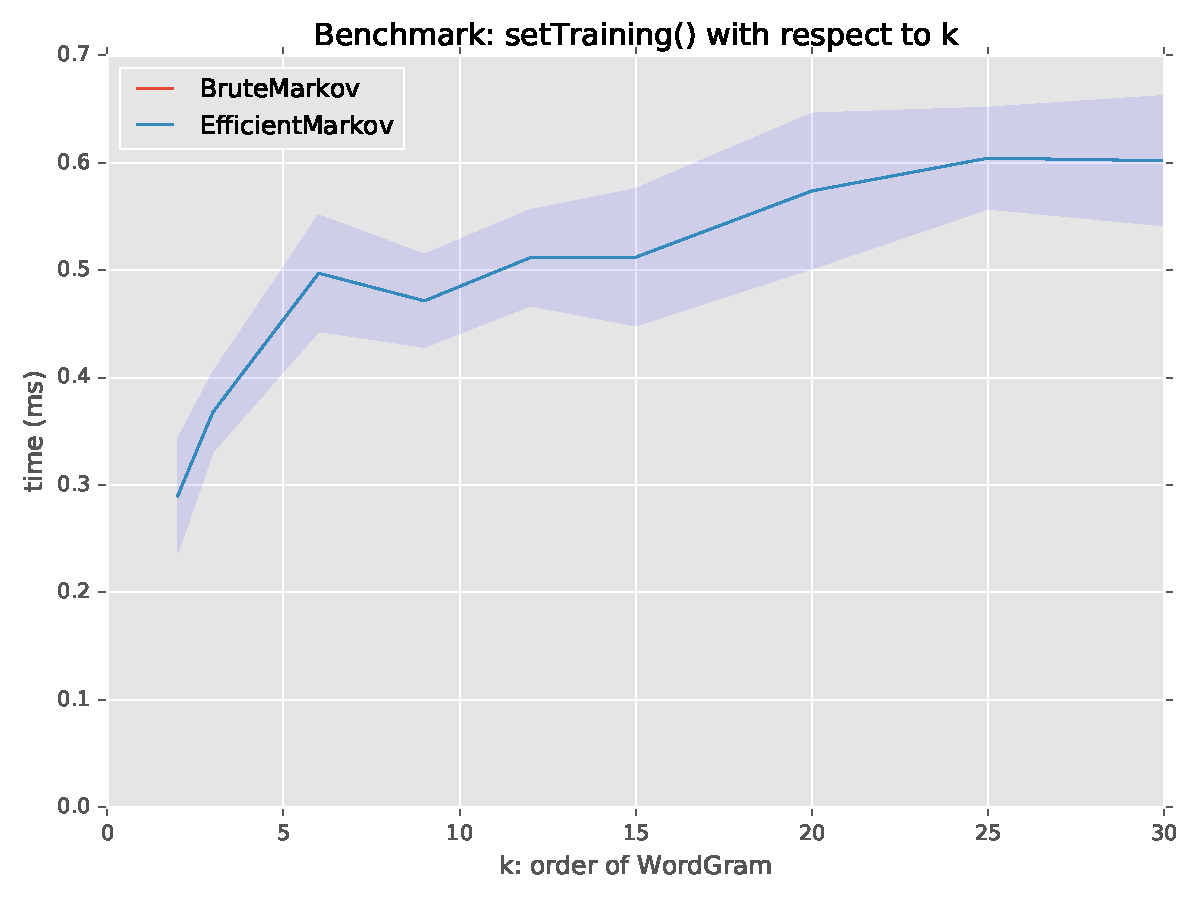
\includegraphics[width=0.6\linewidth]{setTraining_k.pdf}}

\centerline{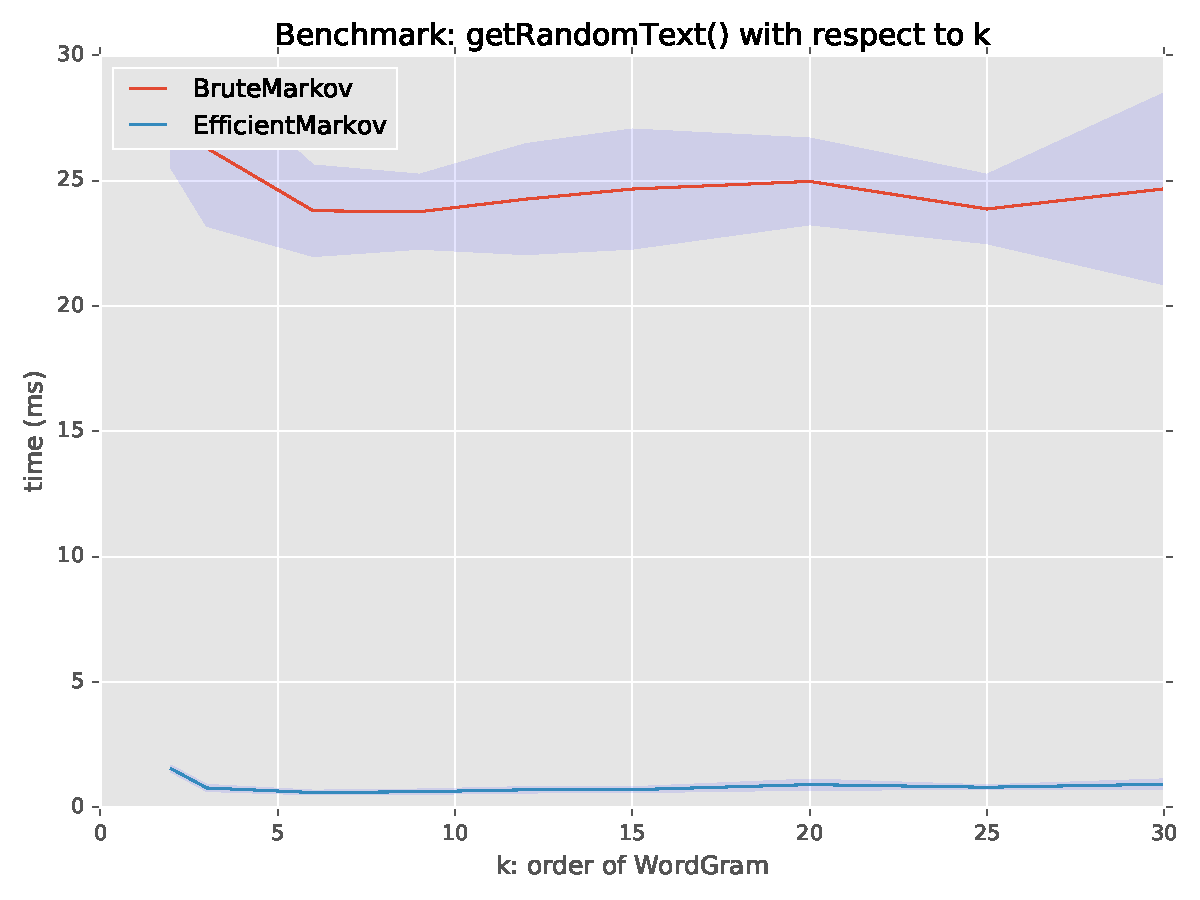
\includegraphics[width=0.6\linewidth]{getRandomText_k.pdf}}

\section{Map Insertion Time Analysis}

Inserting (calling \texttt{\bf .put()} method with) $U$ unique keys is $O(U)$ for \texttt{\bf HashMap} $O(U\log U)$ for \texttt{\bf TreeMap}. Furthermore, I measured the performance for \texttt{\bf IdentityHashMap}. (In Java, \texttt{HashMap} is implemented using separate chaining, storing collisions using a \texttt{LinkedList}, while \texttt{IdentityHashMap} is implemented using linear probing, moving on to the next bucket on collision. Since Java 8, \texttt{HashMap} automatically transforms a bucket that is too huge into a BST.)

\centerline{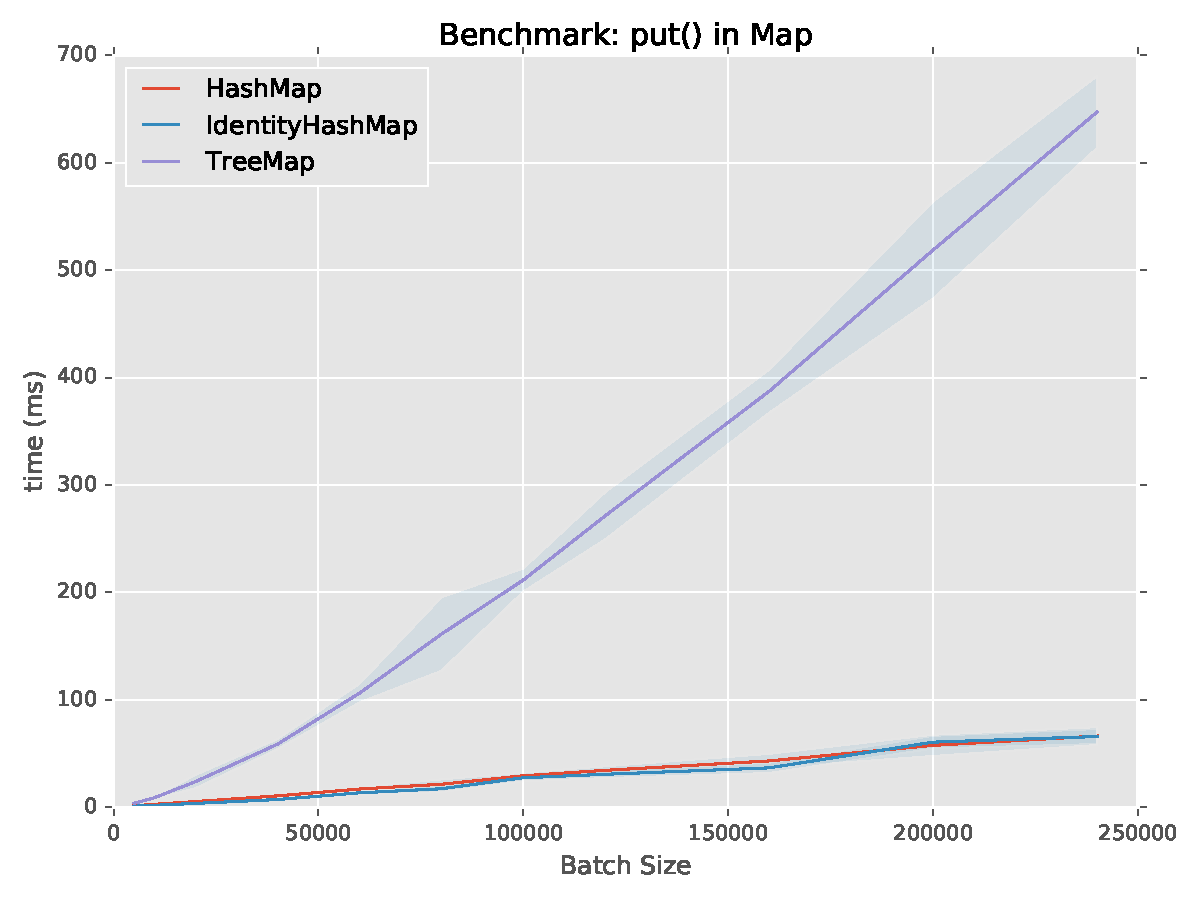
\includegraphics[width=0.6\linewidth]{bench_map_total.pdf}}

\centerline{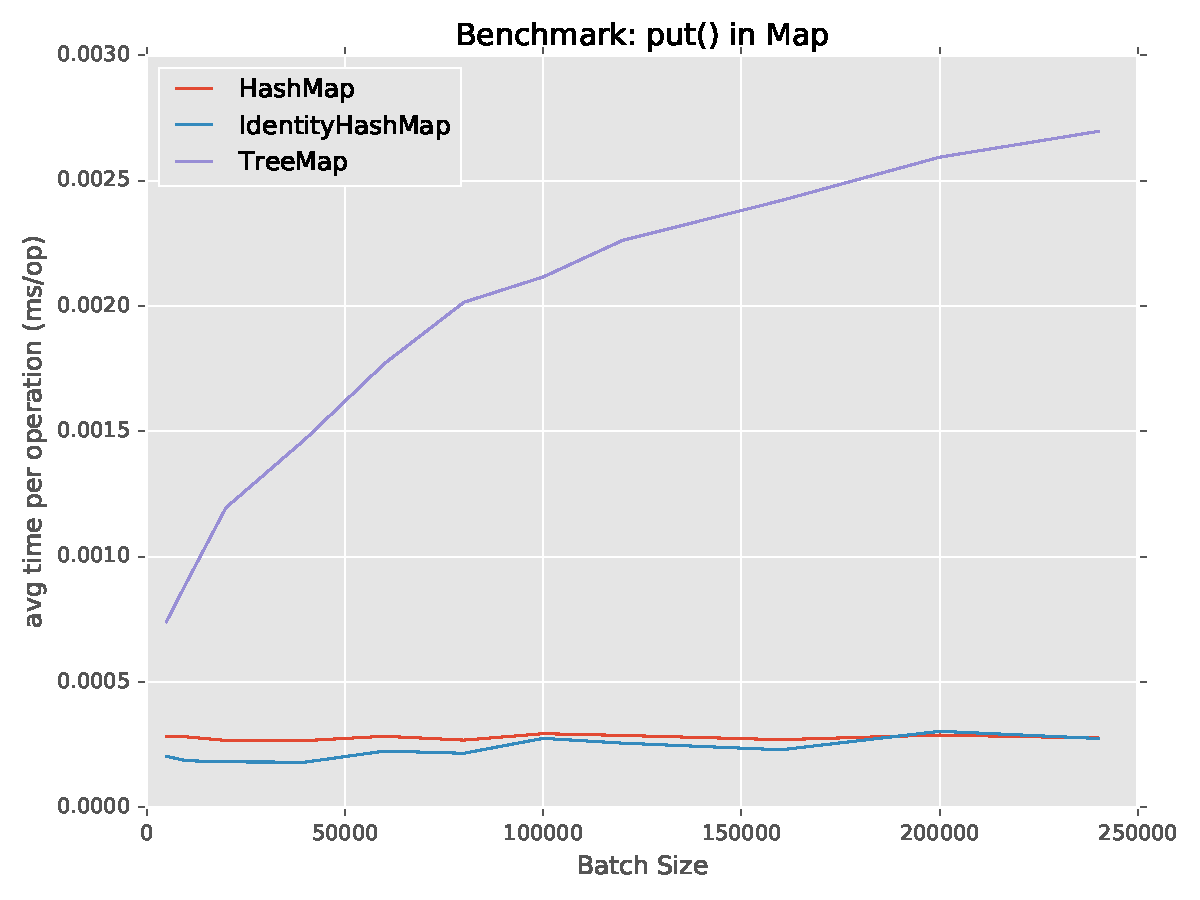
\includegraphics[width=0.6\linewidth]{bench_map_avg.pdf}}

\end{document}